\documentclass[10pt,landscape]{article}
\usepackage{ling}
\usepackage{tikz}
\usepackage{tikz-qtree}
\usetikzlibrary{arrows,decorations.pathmorphing,backgrounds,positioning,fit,matrix,shapes}
\usepackage{txfonts}


\usepackage[hmargin=2cm,vmargin=2cm]{geometry}
\geometry{a4paper}
 
 \usepackage{fancyhdr} % This should be set AFTER setting up the page geometry
 \pagestyle{fancy} % options: empty , plain , fancy
 \renewcommand{\headrulewidth}{0pt} % customise the layout...
 \lhead{}\chead{}\rhead{}
 \lfoot{}\cfoot{\thepage}\rfoot{}
 
 \begin{document}
 	
\begin{figure}
\centering

\newcommand{\putat}[3]{\begin{picture}(0,0)(0,0)\put(#1,#2){#3}\end{picture}}

 	\Large{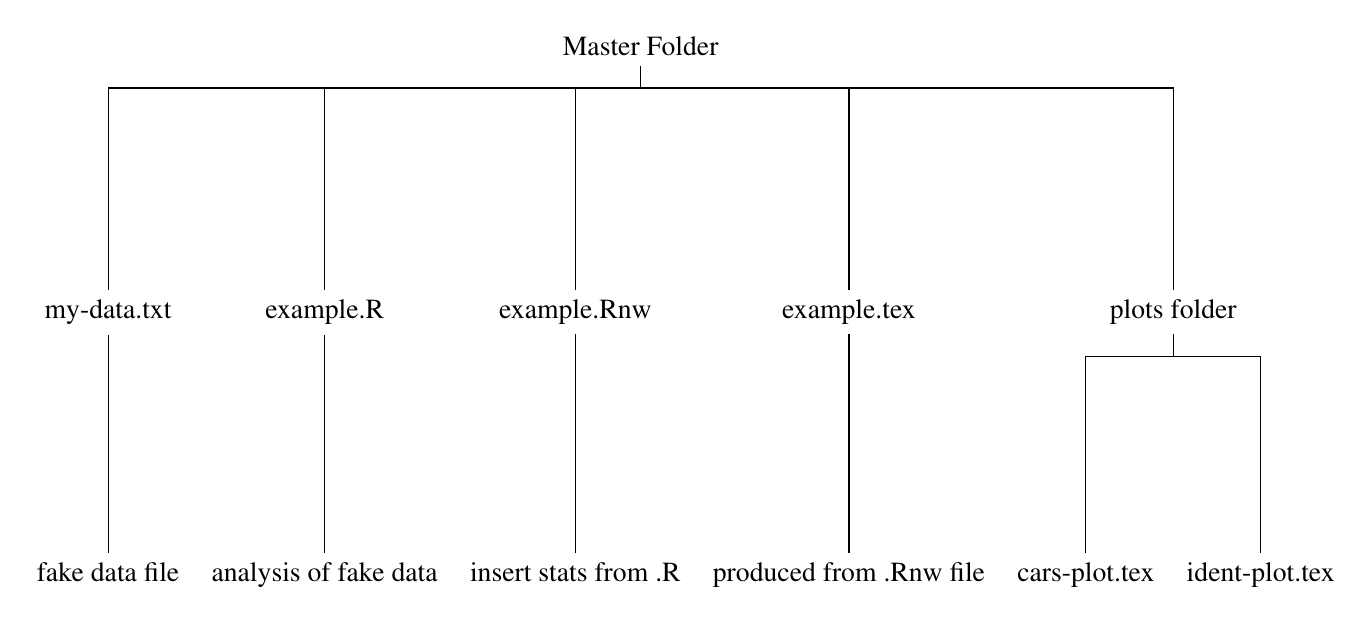
\begin{tikzpicture}%[grow=right]
		\tikzset{level distance=95pt,sibling distance=5pt}
		\tikzset{edge from parent/.style=
			{draw,
				edge from parent path={(\tikzparentnode.south)
					-- +(0,-8pt)
					-| (\tikzchildnode)}}}
		%\tikzset{execute at begin node=\strut}
		\Tree [.{Master Folder} [.{my-data.txt} {fake data file} ] [.{example.R} {analysis of fake data} ] [.{example.Rnw} {insert stats from .R} ] [.{example.tex} {produced from .Rnw file} ] [.{plots folder} {cars-plot.tex} {ident-plot.tex} ] ]
	\end{tikzpicture}}

\end{figure}
 \end{document}